\documentclass[12pt]{article}
\usepackage[a4paper]{geometry}
\usepackage{graphicx}
\usepackage{cleveref}
\title{Kaggles stroke dataset}
\author{Ciaran Welsh}

\begin{document}

    \maketitle

    \section{Introduction}
    I have trained a feed forward neural network to classify people into stroke victims or not-stroke victims
    based on their age, their average glucose level, hypertension, heart disease, gender, bmi, marital status and
    work type.
    \subsection{Exploration}
    After some initial exploration I decided to that the best way to visualise this data is by
    using scatter matrix plots with kernel density estimators along the diagonal. An example is shown in
    \cref{fig:scatter_matrix} which the rest can be found in \<root\>/data/Plots/scatter\_matrix.

    \section{Preprocessing}
    The biggest problem with this dataset is that the number of stroke samples was much smaller than the number
    of non-stroke samples (98\% vs 2\%). To deal with this problem, I chose to under sample the non-stroke
    data such that the numbers of non-stroke sample equals the number of stroke samples in both the training and validation data.
    While a good place to start, this turned out to be a naive approach that disregarded the profound impact that age
    has on the changes of a stroke incident (\cref{fig:scatter_matrix}). Training using this sampling approach resulted in
    a large variation in the model's predictive performance, as evaluated by the performance on validation data. To solve the
    problem I ensured non-stroke samples had the same age distribution as the stroke samples.

    \begin{figure}[t]
        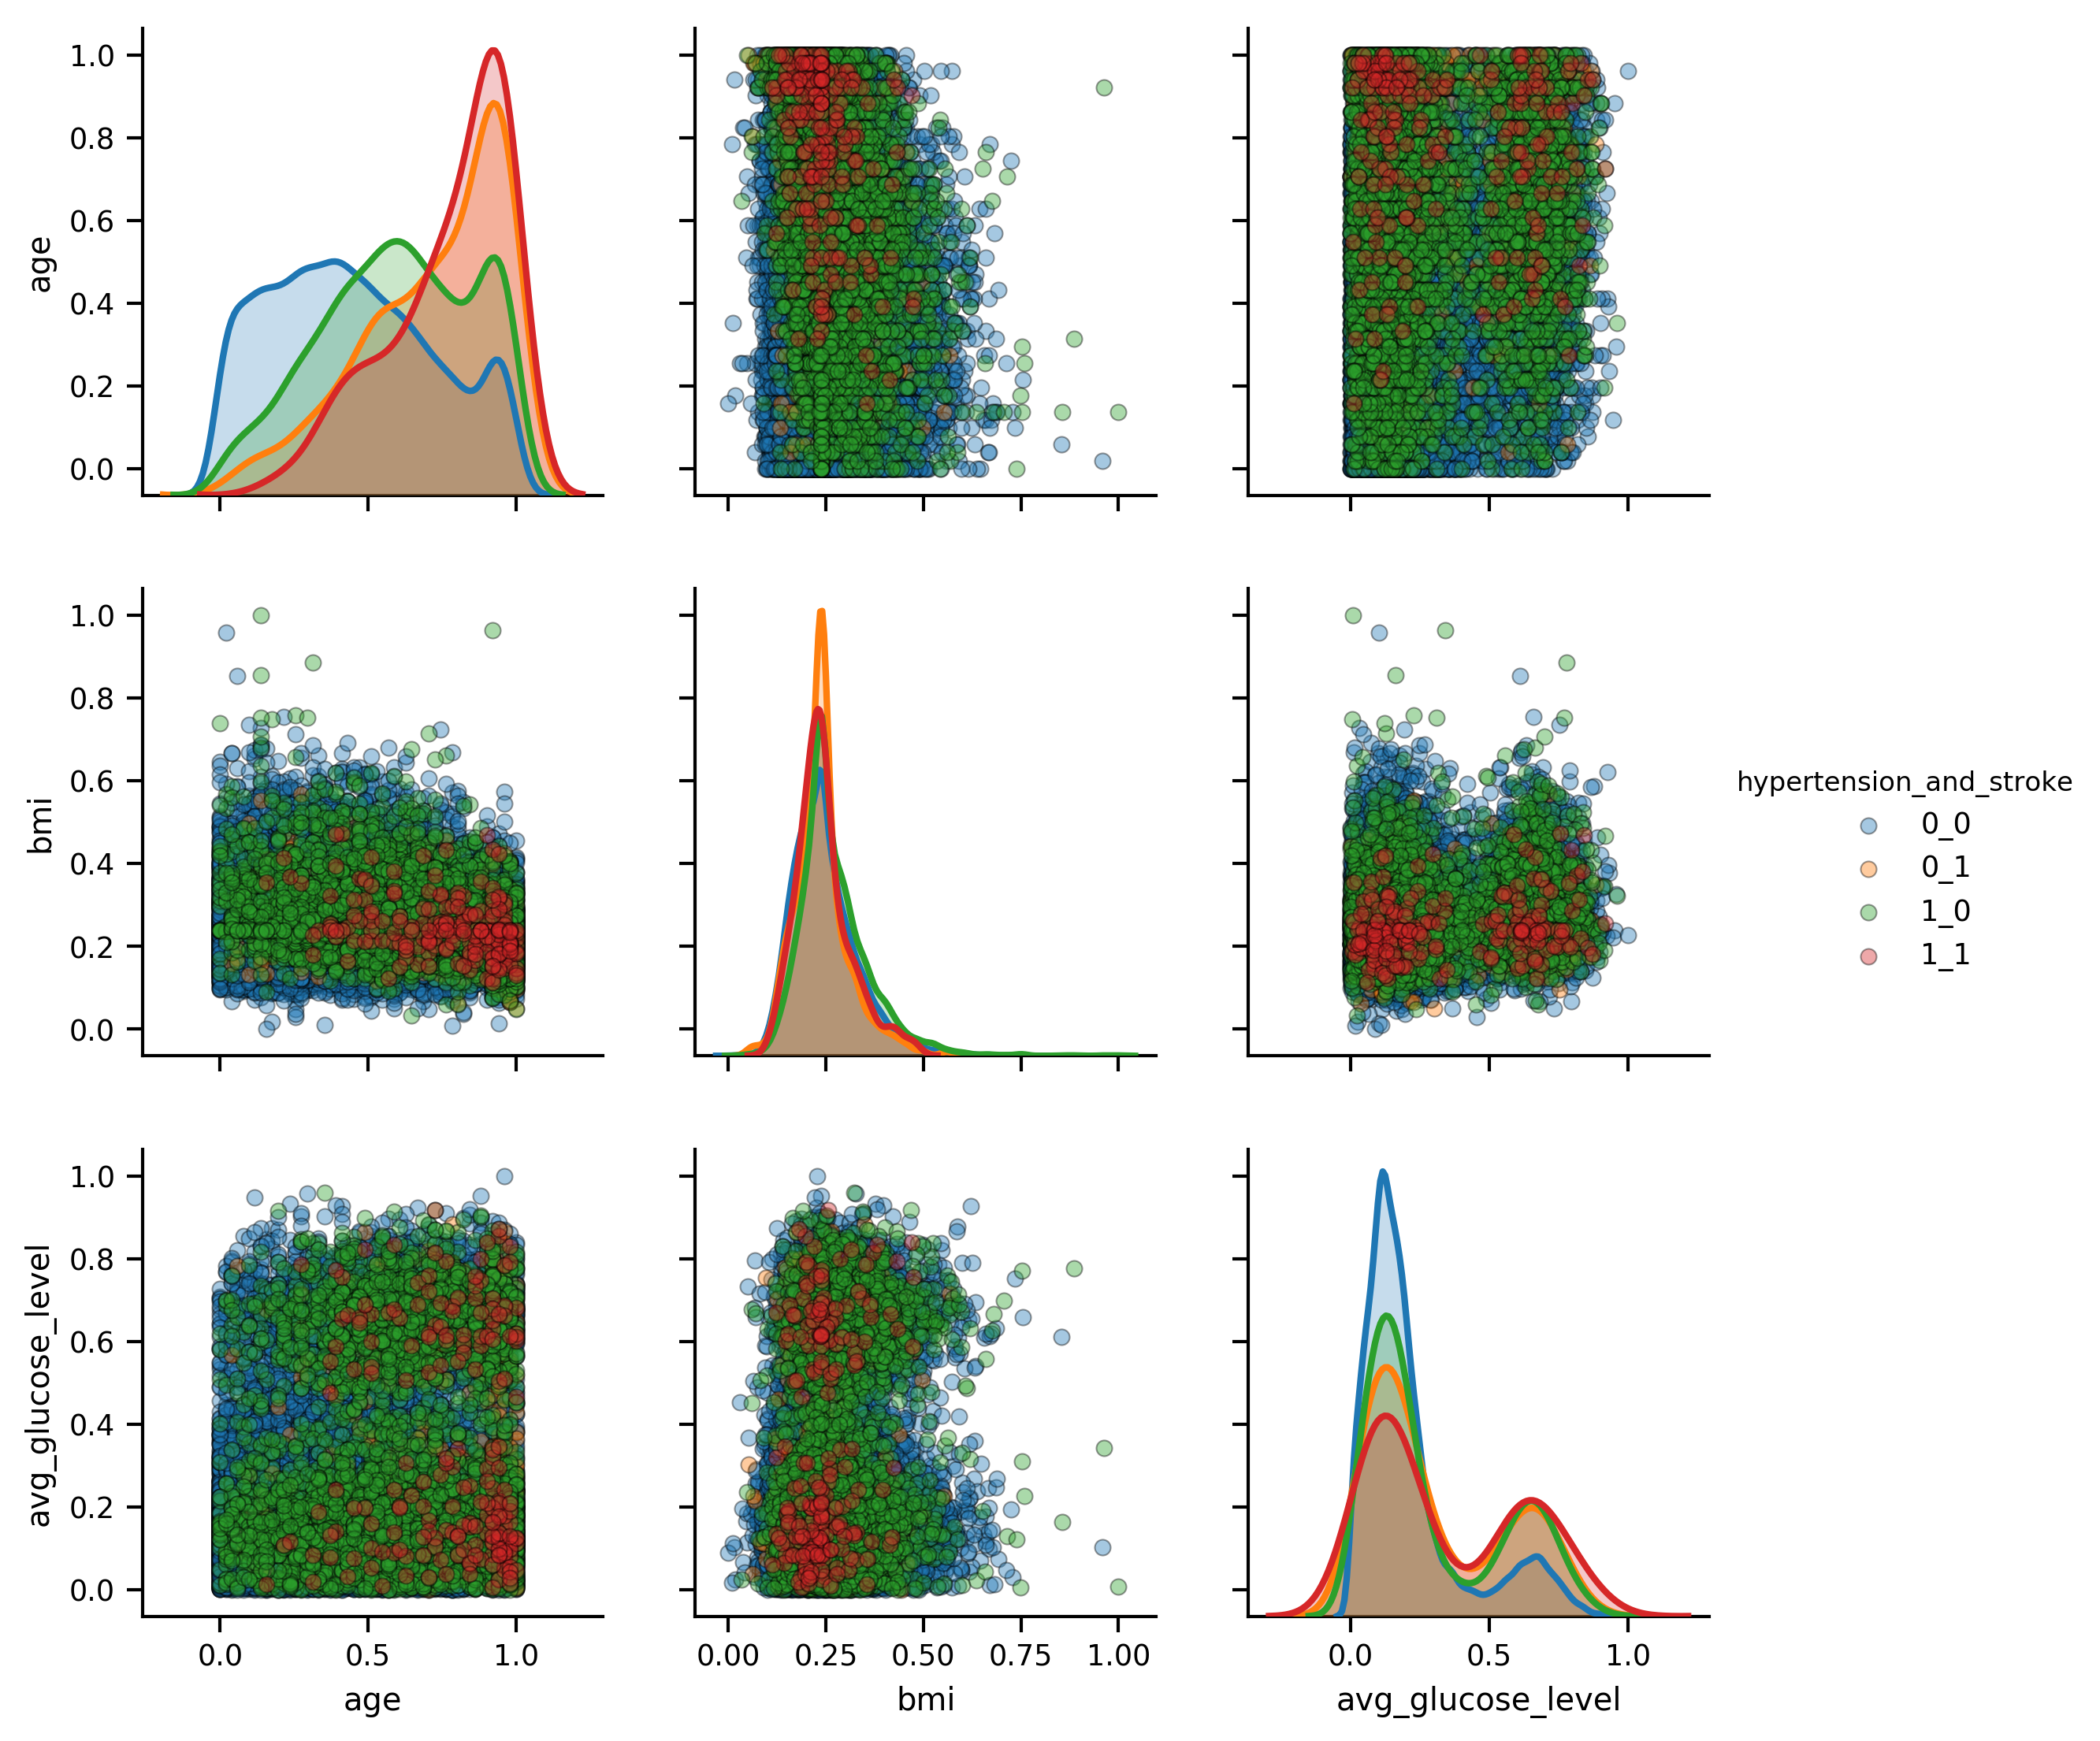
\includegraphics[width=\textwidth]{../data/Plots/scatter_matrix/proc_hypertension.png}
        \caption{Scatter matrix showing relationships between bmi, average glucose levels. This plot is coloured by
        hypertension and stroke}
        \label{fig:scatter_matrix}
    \end{figure}

    Other data preprocessing steps that I used include:
    \begin{enumerate}
        \item Discard young data. There are very few people under 30 in this dataset that have had a stroke. Therefore these were removed from the analysis. Obviously this becomes less important with the age stratified under sampling.
        \item Drop the `other` gender. There are very few `other' values and none who have had strokes.
        \item Impute the bmi column using the median, since only around 3\% of data were missing this is reasonable.
        \item Scale continuous data between 0 and 1 so they exist on a similar scale for fitting
        \item One hot encode categorical  and boolean variables
        \item Remove the residence category: exploratory data analysis seems to suggest its not predictor of stroke incidence.
        \item Remove smoking status category. It has too many missing values to deal with now - maybe of use for model improvement.
        \item Remove any remaining samples with nan values.
    \end{enumerate}

    Note that model performance may still be improved by modifying the preprocessing strategy. There is a
    package called Imbalanced-learn that would be of interest regarding sampling strategy.

    \subsection{Model architecture}
    A simple feedforward network was implemented using the tensorflow.keras interface. Dropout layers were used
    after each dense layer for regularization and the relu activation funciton was used in dense layers. The output layer has a single
    neural with a sigmoid activation function and the model was trained by minimizing the binary crossentropy objective
    function using the ADAM optimizer. An early stopping callback was used to prevent overfitting by stopping training
    when the validation accuracy begins to decline. A plot of training history can be found in \cref{fig:training_history}.

    \begin{figure}
        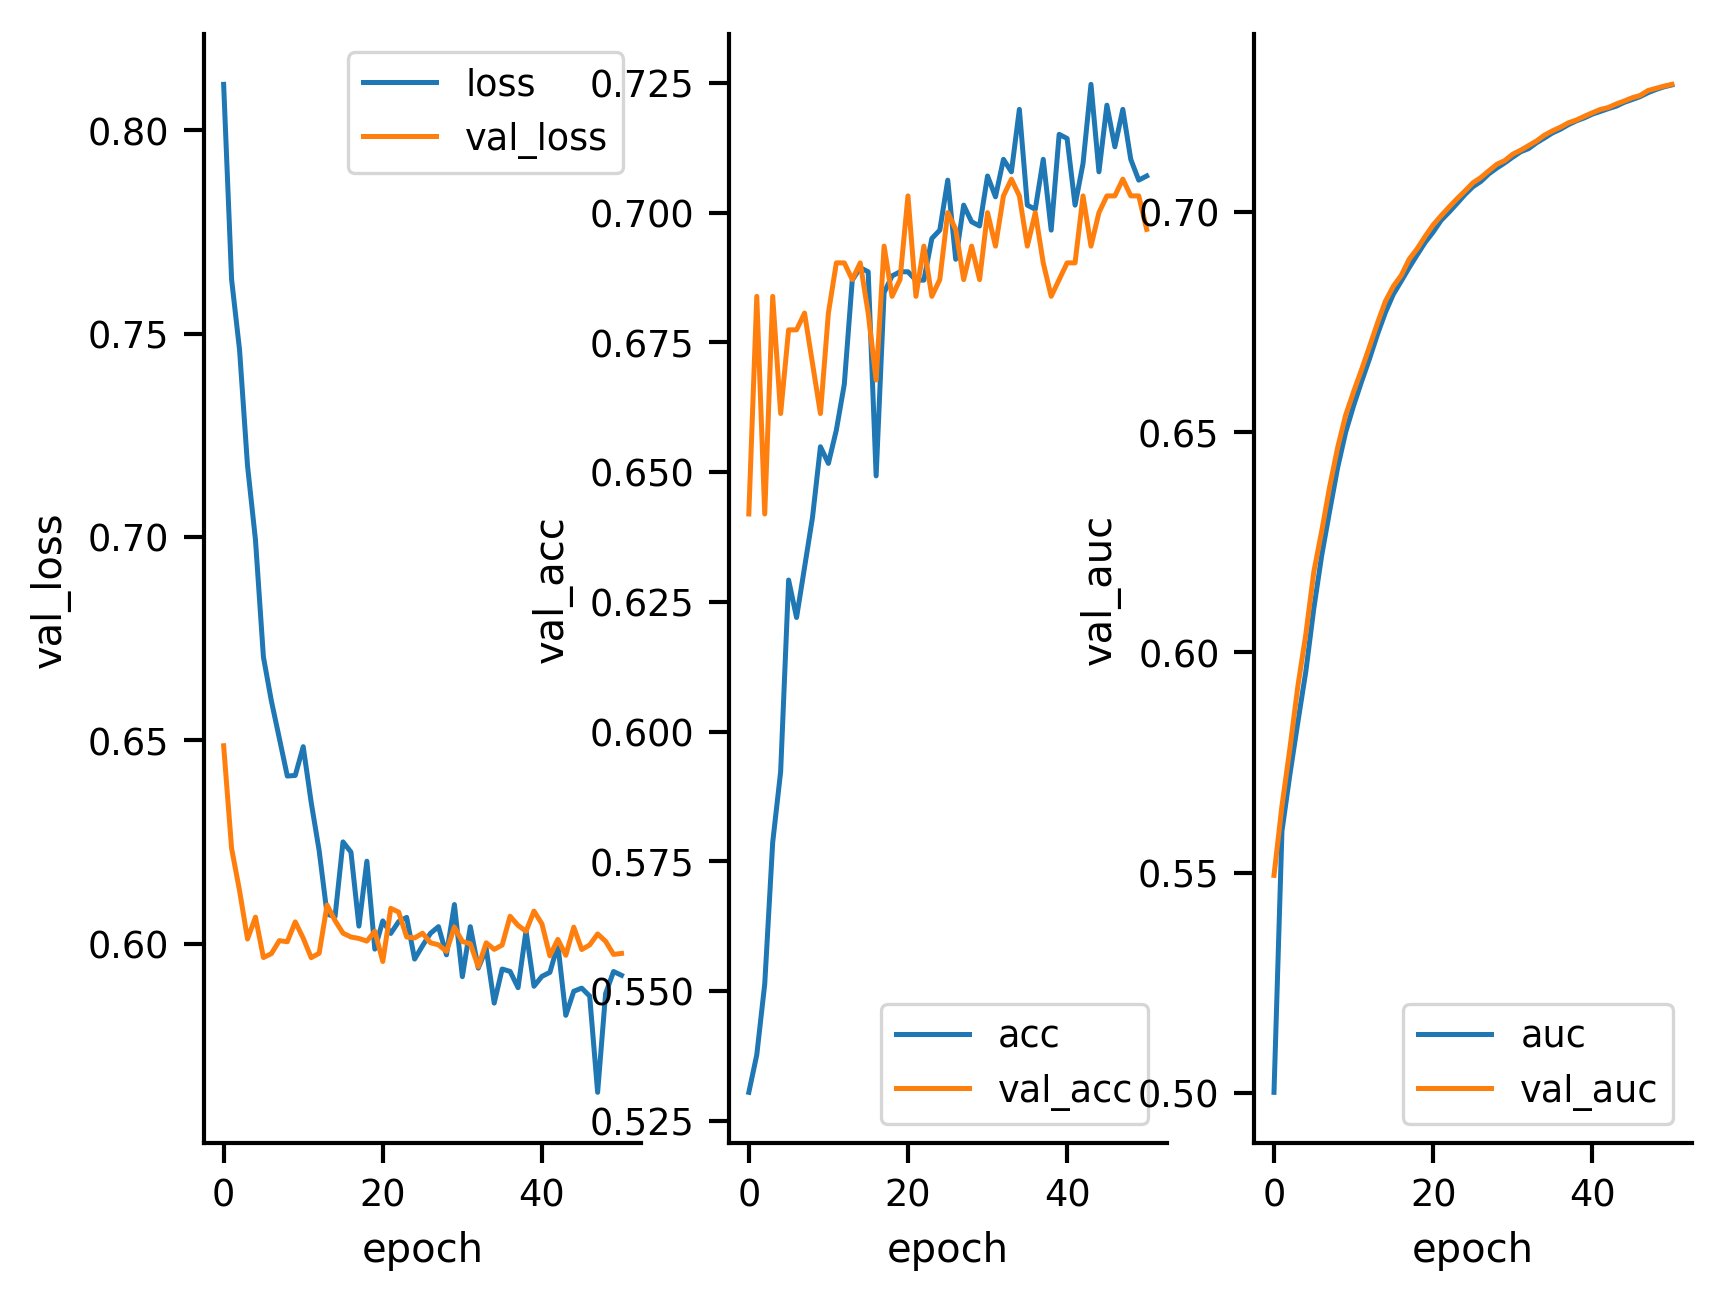
\includegraphics[width=0.75\textwidth]{../data/Plots/history.png}
        \caption{Training history}
        \label{fig:training_history}
    \end{figure}

    \subsection{The model setup}
    Since an under sampling strategy was used to deal with the imbalanced data problem, the model only trains
    with a fraction of the data. To assess the models predictive robustness, a bootstrapping strategy was used (\cref{table:boot}).
    Model train and validation scores were monitored while repeating the model fitting process with a different sample
    from the not-stroke population with the same stroke population. Its possible this decision may have a negative impact
    on model generality due to over fitting the stroke population. As before, sampling was stratified by age group in
    addition to ensuring equal proportions of stroke and not-stroke victim.

    \begin{table}[t]
        \begin{tabular}{|c|c|c|c|c|}
            \hline
            & loss & acc & val\_loss & val\_acc \\ \hline
            Average & 0.61 & 0.70 & 0.59 & 0.71     \\ \hline
            Std & 0.013 & 0.014 & 0.020 & 0.029    \\ \hline
        \end{tabular}
        \caption{Average and standard deviations for 100 bootstrap models}
        \label{table:boot}
    \end{table}

    \subsection{Model Performance}
    Overall, the final model (which I do not have time to improve) has a lot of issues. Even with using age stratified sampling
    the models performance fluctuates a lot, albeit far less than without age stratified sampling. This probably indicates that
    much of the samples are being categorised randomly, and therefore prone to rapid class switching between epochs. While the bootstrapping
    procedure indicates that the model robustly correctly classifies around 70\% accuracy on the validation data, this result is
    probably confounded by the patience parameter of the early stopping procedure. Overall its clear that this model isn't training well
    and changes are required to make it perform better.

    Solutions for a better classifier include modifying better feature selection. It would be valuable to train a model
    multiple times while dropping each variable in turn to measure the variables impact on stroke prediction. The contineous variables
    were scaled to be between 0 and 1, an alternative scaling method may yield better results. From preliminary simulations,
    I've ascertained that modifications to the model architecture does not significantly change the model performance and therefore
    changes to the input data may be a better strategy for taking this model forward.


\end{document}

% However, I am not convinced that all of these variables are informative for classifying stroke victims.
%    I have already excluded residence as a factor involved in stroke incidence based on the scatter plot (data/Plots/scatter_matrix/raw_Residence_type)
%    but I suspect marital status should be excluded as well. Given more time I would systematically drop each variable
%    in turn and measure its impact on model performance.
%